% Beamer slide template prepared by Tom Clark <tom.clark@op.ac.nz>
% Otago Polytechnic
% Dec 2012

\documentclass[10pt]{beamer}
\usetheme{Dunedin}
\usepackage{graphicx}
\usepackage{fancyvrb}

\newcommand\codeHighlight[1]{\textcolor[rgb]{1,0,0}{\textbf{#1}}}

\title{The Decorator Pattern and Python Decorators}

\author[IN608]{Intermediate Application Development}
\institute[Otago Polytechnic]{
  Otago Polytechnic \\
  Dunedin, New Zealand \\
  Kaiako: Tom Clark
}
\date{}
\begin{document}

%----------- titlepage ----------------------------------------------%
\begin{frame}[plain]
  \titlepage
\end{frame}

%----------- slide --------------------------------------------------%
\begin{frame}
  \frametitle{Introduction}
  
  In this session we will see the classic \emph{Decorator} pattern 
  from GoF. We also also look that the Python language feature with 
  the same name and compare and contrast them.
  
\end{frame}

%----------- slide --------------------------------------------------%
\begin{frame}
  \frametitle{Decorator Intent}
  
  ``Attach additional responsibilities to an object dynamically. Decorators
  provide a flexible alternative to subclassing for extending functionality'' \\
  (\emph{GoF})
  
  \vspace{5mm}
  The typical way to extend or modify a class's behaviour is to subclass it. But this 
  modification is locked in at compile time. Sometimes we want to wait until runtime to apply 
  the modification, perhaps to apply it selectively.
  

  
\end{frame}

%----------- slide --------------------------------------------------%
\begin{frame}
  \frametitle{An Example}
  
  When a player of one of Runaway's games is having trouble and raises a support issue,
  we enable extra logging of that player's API calls. Then, at runtime we modify the behaviour of
  API calls \emph{Just for that player}, to log the details of the calls.
       
\end{frame}

%----------- slide --------------------------------------------------%
\begin{frame}
  \frametitle{The Plan}
  
  Start with a standard instance of a class, \texttt{basic}. From here we
  
  \begin{itemize}
    \item Construct a decorator instance that ``wraps'' basic.
    \item This decorator instance presents the same interface as \texttt{basic}, making it a replacement.
    \item However, the decorator can take over some of \texttt{basic}'s methods, while also leaving some unchanged.
    \item We can also recover the undecorated \texttt{basic} instance. It is unchanged by the process.
    \item Also, we can selectively choose whether to apply the decorator, or choose from a range of decorators to apply.
  \end{itemize}

  \end{frame}
%----------- slide --------------------------------------------------%
\begin{frame}
  \frametitle{Structural Diagram} 
  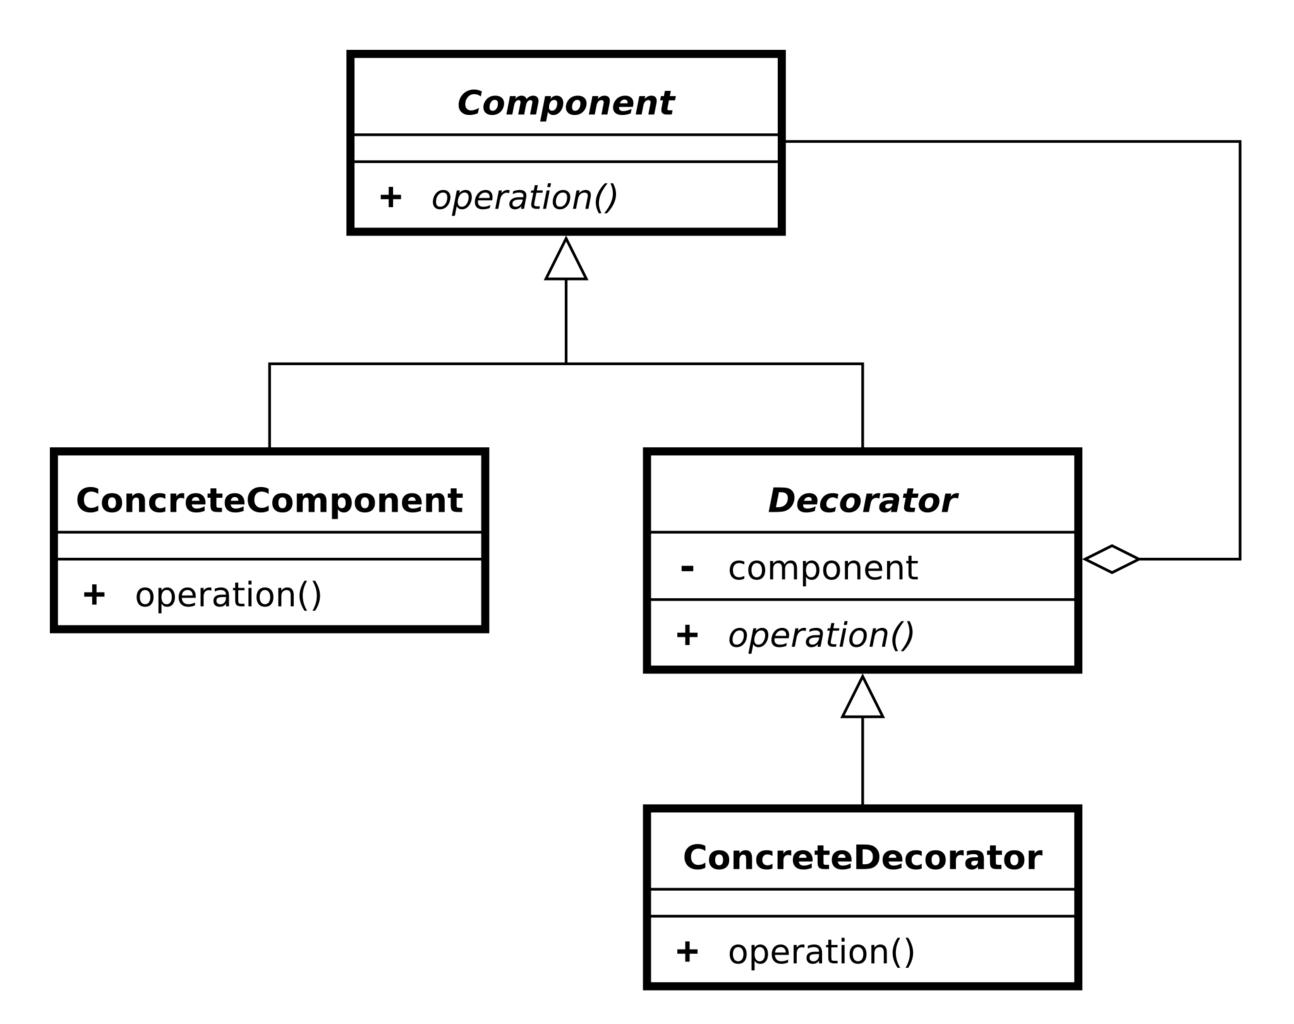
\includegraphics[width=8cm]{decorator.jpg}
  \end{frame}

%----------- slide --------------------------------------------------%
\begin{frame}[fragile]
  \frametitle{Decorator Implementation: Base }

  \begin{verbatim}
  from abc import ABC, abstractmethod
  
  class AbstractMessenger(ABC):
  
    @abstractmethod
    def say_hello(self):
        pass

    @abstractmethod
    def say_goodbye(self):
        pass

    @abstractmethod
    def tell_the_time(self):
        pass
        
  
  \end{verbatim}
 \end{frame} 
 
 %----------- slide --------------------------------------------------%
\begin{frame}[fragile]
  \frametitle{Decorator Implementation: Concrete Subclass }

  \begin{verbatim}
   class ConcreteMessenger(AbstractMessenger):

     def say_hello(self):
         return 'Hello'

     def say_goodbye(self):
         return 'Goodbye'

     def tell_the_time(self):
         return datetime.now()

  \end{verbatim}
 \end{frame} 

 %----------- slide --------------------------------------------------%
\begin{frame}[fragile]
  \frametitle{Decorator Implementation: Decorators }

  \begin{verbatim}
  class AbstractDecorator(AbstractMessenger):
   
    def __init__(self, messenger):
        self._messenger = messenger

    def tell_the_time(self):
        return self._messenger.tell_the_time()
        
  class UppercaseDecorator(AbstractDecorator):
  
    def say_hello(self):
        msg = self._messenger.say_hello()
        return msg.upper()

    def say_goodbye(self):
        msg = self._messenger.say_goodbye()
        return msg.upper()      
  \end{verbatim}
 \end{frame} 

 %----------- slide --------------------------------------------------%
\begin{frame}[fragile]
  \frametitle{Decorator Implementation: In Use}

  \begin{verbatim}
  basic_messenger = ConcreteMessenger()
  print(basic_messenger.say_hello()) # prints 'Hello'
  
  upper_messenger = UppercaseDecorator(basic_messenger)
  print(upper_messenger.say_hello()) # prints 'HELLO'
  \end{verbatim}
 \end{frame} 


 %----------- slide --------------------------------------------------%
\begin{frame}
  \frametitle{Programming Activity}
  
  \begin{enumerate}
    \item Pull the course materials repo.
    \item Create a new branch, \texttt{11-practical} in your practicals repo.
    \item Add a subdirectory,  \texttt{11-practical} and copy \texttt{11-practical.ipynb} from the class materials into it.
    \item Open a shell, cd to this directory, and run \texttt{jupyter notebook} to open the notebook. Complete the first two questions.
    \item We will discuss results in 20ish minutes.
  \end{enumerate}      
\end{frame}

%----------- slide --------------------------------------------------%
\begin{frame}[fragile]
  \frametitle{Python Decorators}
  Python has a core language feature called a decorator. You've seen them already.
  
  \vspace{5mm}
  \begin{Verbatim}[commandchars=\\\{\}]
    \codeHighlight{@abstractmethod}
    def say_hello(self):
        pass
        
  \end{Verbatim}
  A lot of literature on the topic will go out of its way to point out that 
  Python decorators are not the same thing as the Decorator pattern. Except 
  they kind of are. I mean, they're not... but sometimes they are.      
\end{frame} 

%----------- slide --------------------------------------------------%
\begin{frame}[fragile]
  \frametitle{Decorating Functions}
  In practice, Python decorators are usually applied to functions
  rather than clases, although we definitely can decorate classes. 
  
  \vspace{5mm}
  \begin{Verbatim}[commandchars=\\\{\}]
    \codeHighlight{@abstractmethod}
    def say_hello(self):
        pass
        
  \end{Verbatim}
  There are many decorators built into the language or provided in the standard library.
  We've already seen some like \texttt{@property} and \texttt{@classmethod}.    
\end{frame} 

%----------- slide --------------------------------------------------%
\begin{frame}[fragile]
  \frametitle{Implementing a Decorator}
  A function decorator generally ``wraps'' a function and returns a modified version of that function.  
  \vspace{5mm}
  \begin{verbatim}
  import functools
  
  def shouty(wrapped_fn):
      @functools.wraps(wrapped_fn)
      def wrapper(*args, **kwargs):
          msg = wrapped_fn(*args, **kwargs)
          return msg.upper()
      return wrapper
  
  #usage:    
  @shouty
  def hello():
      return 'hello' 
      
  hello() #prints 'HELLO'           
  
  \end{verbatim}
  
\end{frame} 

%----------- slide --------------------------------------------------%
\begin{frame}[fragile]
  \frametitle{Decorators With Arguments}
  A function decorator generally ``wraps'' a function and returns a modified version of that function.  
  \vspace{5mm}
  \begin{verbatim}
  def shouty_or_not(choice):
      def maybe(wrapped_fn):
          @functools.wraps(wrapped_fn)
          def wrapper(*args, **kwargs):
              msg = wrapped_fn(*args, **kwargs)
              if choice:
                return msg.upper()
              else:
                return msg  
          return wrapper
      return maybe  
   #usage:
   @shouty_or_not(True)
   def hello():
       return 'hello'   
   \end{verbatim}
  
\end{frame} 

\begin{frame}[fragile]
  \frametitle{A Class Decorator}
  
  \emph{Real Python} has a nice example of a class decorator that make a class into 
  a Singleton.
  
  \vspace{5mm}
  \begin{verbatim}
  https://realpython.com/primer-on-python-decorators/
  #creating-singletons
  \end{verbatim}
\end{frame}

\begin{frame}
  \frametitle{Conclusions}
  
  ``Attach additional responsibilities to an object dynamically. Decorators
  provide a flexible alternative to subclassing for extending functionality'' \\
  (\emph{GoF})

  \begin{itemize}
    \item Python decorators have several uses, some of which don't satisfy this intent.
    \item They also have uses that \textbf{look} very different in their implementation than don't
    look like the textbook pattern, but nonetheless \textbf{do} satisfy the intent.
    \item Regardless of this, Python decorators are handy and widely used.
  \end{itemize}
\end{frame}

\end{document}
